\documentclass[paper=a4, twoside=false, fontsize=12pt, parskip=half,
                bibliography=totoc, listof=totoc]{scrbook}

% General packages
\usepackage{pgfplots}
\usepackage{fontspec}
\usepackage[mode=match, reset-text-family=false]{siunitx}
\usepackage{fontspec}
\usepackage{calc}
\definecolor{codeblue}{RGB}{69, 161, 248}
\definecolor{codeblack}{RGB}{40, 40, 40}

\definecolor{maingray}{HTML}{F8F8F8}

\definecolor{hlocre}{HTML}{E5B874}
\definecolor{hlorange}{HTML}{EC7850}
\definecolor{hlyellow}{HTML}{FAE69E}

\definecolor{pinkpic}{RGB}{246, 183, 194}
\definecolor{redpic}{RGB}{232, 72, 71}
\definecolor{yellowpic}{RGB}{246, 235, 51}

% Define flowcharts macros independently so we can build them as png files
% for the website or something. This is supported in the makefile
\tikzstyle{every picture}+=[font=\footnotesize\sffamily]
\usetikzlibrary{calc, shapes, arrows, decorations.pathreplacing, calligraphy,
                calligraphy}
\tikzstyle{decision} = [diamond, draw=codeblack, fill=codeblack, text=white,
    text width=4.5em, text badly centered, node distance=3cm, inner sep=0pt,
    line width=2mm]
\tikzstyle{block} = [rectangle, draw=codeblack, fill=white,  text=black,
    text width=5em, text centered, rounded corners, minimum height=4em,
    line width=0.4mm]
\tikzstyle{decision_start} = [diamond, draw=codeblack, fill=pinkpic, text=black,
    text width=4.5em, text badly centered, node distance=3cm, inner sep=0pt,
    line width=0.4mm]
\tikzstyle{start} = [rectangle, draw=codeblack, fill=pinkpic,  text=black,
    text width=5em, text centered, rounded corners, minimum height=4em,
    line width=0.4mm]
\tikzstyle{success} = [rectangle, draw=codeblack, fill=yellowpic,  text=black,
    text width=5em, text centered, rounded corners, minimum height=4em,
    line width=0.4mm]
\tikzstyle{fail} = [rectangle, draw=codeblack, fill=redpic,  text=black,
    text width=5em, text centered, rounded corners, minimum height=4em,
    line width=0.4mm]
\tikzstyle{line} = [draw, -latex', thick, ->,>=to]

\tikzstyle{BC} =  [decorate,  % Brace Calligraphic
                 decoration={calligraphic brace, amplitude=3mm, raise=1mm},
                 very thick, pen colour={black} ]
\tikzstyle{loop} = [arc, draw=codeblack, line width=0.4mm]

\tikzstyle{timeline_event}=[align=center, fill=white, inner sep=2pt]

\tikzstyle{timeline_timespan} = [rectangle, draw=codeblack, fill=pinkpic,  text=black,
    text centered, rounded corners, line width=0.4mm]

% Fonts
\defaultfontfeatures{Scale=MatchLowercase, Ligatures=TeX}
% Define Semi-bold
\DeclareRobustCommand\sbseries{\fontseries{sb}\selectfont}
% Fonts for accessibility
\ifdefined\isaccessible
    \setmainfont{Open Sans}[
    Scale=MatchLowercase]
\else
    \setmainfont{TeX Gyre Pagella}[Scale=1.0] % Or Palatino Linotype, etc.
    % TODO not available on github CI
    % \setmonofont{Andale Mono}[Scale=MatchLowercase]
\fi
% Opens Sans in both case..
\setsansfont{Open Sans}[
  Scale=MatchLowercase,
  FontFace = {sb}{it}{* Semibold Italic},
  FontFace = {sb}{n}{*-semibold}]
\usepackage{layouts}

\newcommand{\printsizes}{
    Width: \printinunitsof{in}\prntlen{\textwidth}in \\
    Height: \printinunitsof{in}\prntlen{\textheight}in
}

\begin{document}
\begin{figure}[!htb]
  \centering
  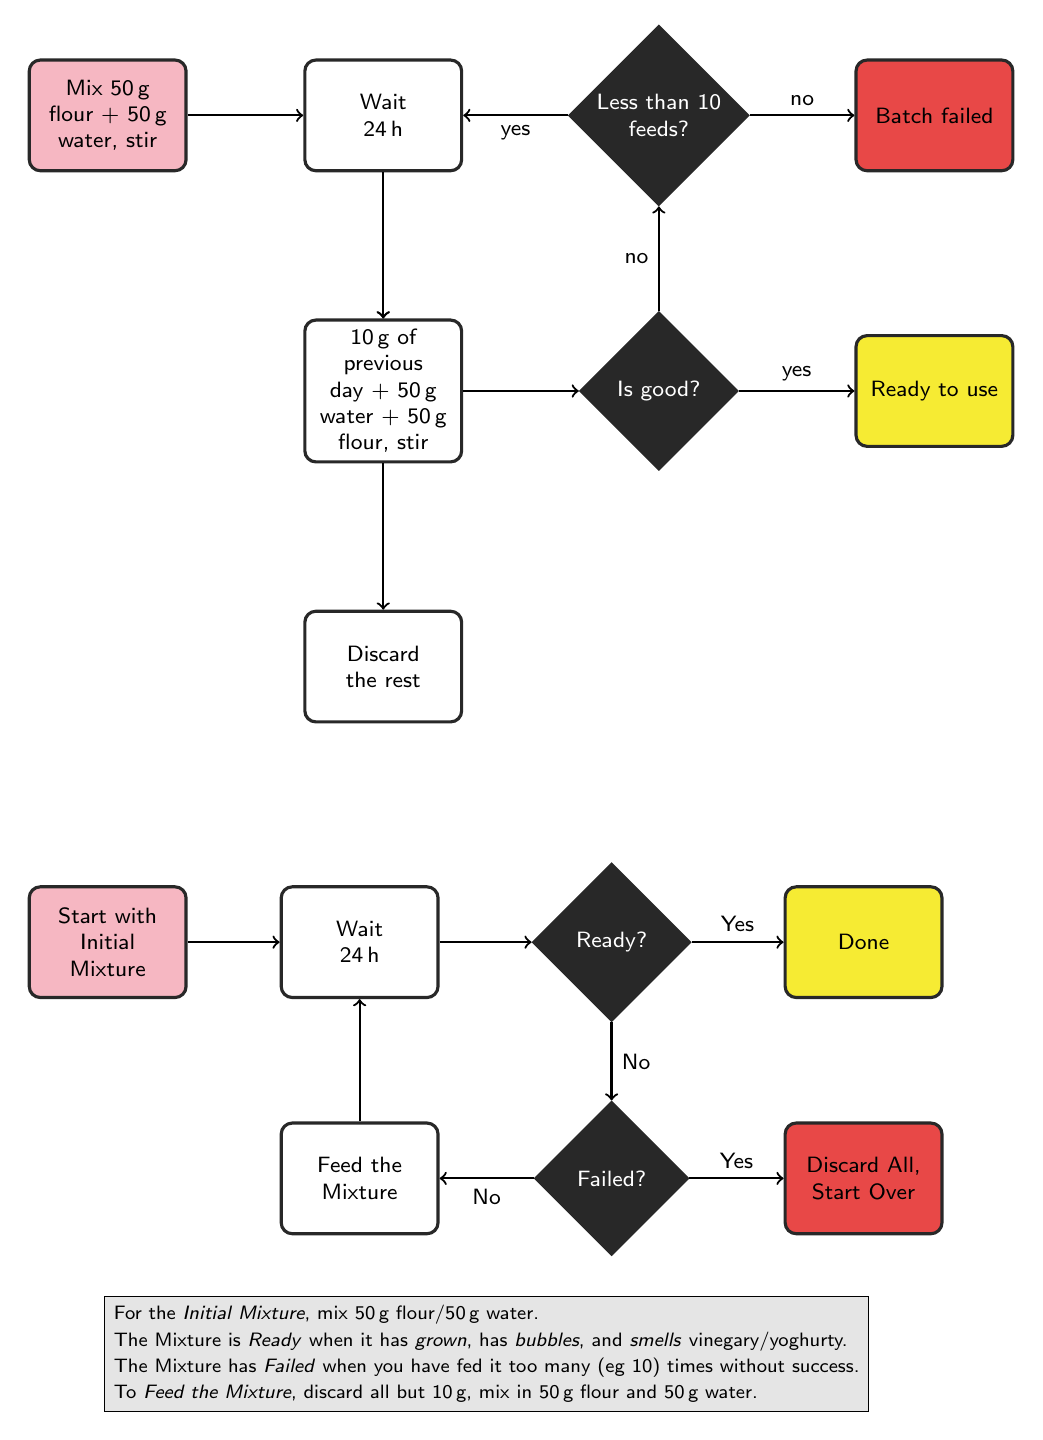
\begin{tikzpicture}[node distance = 3.5cm, auto]
  \node [start] (init) {Mix \qty{50}{\gram} flour + \qty{50}{\gram} water, stir};
  \node [block, right of=init] (wait2) {Wait\\ \qty{24}{\hour}};
  \path [line] (init) -- (wait2);
  \node [block, below of=wait2, node distance=3.5cm] (feed) {\qty{10}{\gram} of previous day + \qty{50}{\gram} water + \qty{50}{\gram} flour, stir};
  \path [line] (wait2) -- (feed);
  \node [block, below of=feed] (discard) {Discard the rest};
  \path [line] (feed) -- (discard);
  \node [decision, right of=feed, node distance=3.5cm] (decide) {Is good?};
  \node [decision, above of=decide, node distance=3.5cm] (timeout) {Less than 10 feeds?};
  \node [fail, right of=timeout, node distance=3.5cm] (discard2) {Batch failed};
  \path [line] (timeout) -- node{no} (discard2);
  \path [line] (timeout) -- node{yes} (wait2);
  \path [line] (feed) -- (decide);
  \node [success, right of=decide, node distance=3.5cm] (use) {Ready to use};
  \path [line] (decide) -- node{no} (timeout);
  \path [line] (wait2) -- (feed);
  \path [line] (decide) -- node{yes} (use);

  \node [start, below of=discard, left of=discard] (start_n) { Start with Initial Mixture };
  \node [block, right of=start_n, node distance = 3.2cm] (wait_n) { Wait\\ \qty{24}{\hour} };
  \node [decision, right of=wait_n, node distance = 3.2cm] (readycheck_n) { Ready? };
  \node [block, below of=wait_n, node distance = 3cm] (feed_n) { Feed the Mixture };
  \node [decision, right of=feed_n, node distance = 3.2cm] (limitcheck_n) { Failed? };
  \node [fail, right of=limitcheck_n, node distance = 3.2cm] (abort_n) { Discard All, Start Over };
  \node [success, right of=readycheck_n, node distance = 3.2cm] (final_n) { Done };

  \draw [line] (start_n) -- (wait_n);
  \draw [line] (wait_n) -- (readycheck_n);
  \draw [line] (feed_n) -- (wait_n);
  \draw [line] (readycheck_n) -- node { No } (limitcheck_n);
  \draw [line] (limitcheck_n) -- node (feedok_n) { No } (feed_n) ;
  \draw [line] (limitcheck_n) -- node { Yes } (abort_n);
  \draw [line] (readycheck_n) -- node { Yes } (final_n);

  \node [below of=feedok_n, node distance=2cm, align=left] (details2) [shape=rectangle,draw,fill=white!90!black]{
    \fontsize{7}{9}\selectfont For the \emph{Initial Mixture}, mix \qty{50}{\gram} flour/\qty{50}{\gram} water.\\
    \fontsize{7}{9}\selectfont The Mixture is \emph{Ready} when it has
    \emph{grown}, has \emph{bubbles}, and \emph{smells}
    vinegary/yoghurty. \\

    \fontsize{7}{9}\selectfont The Mixture has \emph{Failed} when you
    have fed it too many (eg 10) times without success.\\

    \fontsize{7}{9}\selectfont To \emph{Feed the Mixture}, discard all but \qty{10}{\gram}, mix in \qty{50}{\gram} flour and \qty{50}{\gram} water.
  };
\end{tikzpicture}

  \caption[Dough strength over time with kneading]{A schematic visualization
      of gluten development in sourdoughs with different kneading techniques.
      A combination of techniques can be utilized to achieve maximum dough
      strength.}%
  \label{fig:dough-strength-sourdough}
\end{figure}
\end{document}
